\documentclass[twocolumn,preprintnumbers,amsmath,amssymb,superscriptaddress]{revtex4}
%\usepackage[pdftex]{graphicx}

\usepackage{amsmath,amsfonts,amssymb}
\usepackage[english]{babel}
\usepackage[latin1]{inputenc}
\usepackage[T1]{fontenc}
\usepackage{color}
\usepackage{float}
\usepackage{verbatim}
\usepackage{graphicx}
\usepackage{bm}
\usepackage{mathtools}
\usepackage{stmaryrd}
\usepackage{anyfontsize}


%\usepackage{epstopdf}
%\usepackage{array}
%\usepackage{tabularx}
%\usepackage{multirow}
\usepackage{color}
%\usepackage{multibox}
%\usepackage{rotating}
%\usepackage{lineno}
%\usepackage[left]{lineno}
\usepackage[comma,sort&compress]{natbib}
\bibpunct{}{}{,}{s}{}{;}
%\usepackage{authblk}
%\usepackage{multicol}

\bibliographystyle{naturemag}

\usepackage{bibunits}

%\linenumbers
%\setlength\linenumbersep{3pt}

\begin{document}


\author{Justin D. Yeakel} \affiliation{School of Natural Sciences, University
  of California, Merced, Merced, CA 95340, USA}\affiliation{The Santa Fe Institute, 1399 Hyde Park Road, Santa Fe, NM 87501, USA}\affiliation{Contributed equally}\affiliation{Corresponding author: jdyeakel@gmail.com}

\author{Christopher P. Kempes} \affiliation{The Santa Fe Institute, 1399 Hyde
  Park Road, Santa Fe, NM 87501, USA}\affiliation{Contributed equally}

\author{Sidney Redner} \affiliation{The Santa Fe Institute, 1399 Hyde Park
  Road, Santa Fe, NM 87501, USA}\affiliation{Contributed equally}

\title{The dynamics of starvation and recovery}%: Eco-evolutionary feedbacks}


\begin{abstract} %250 words
The eco-evolutionary dynamics of species are fundamentally linked to the energetic constraints of its constituent individuals. 
Of particular importance are the tradeoffs between reproduction and the dynamics of starvation and recovery. % in resource-limited environments
We introduce a minimal nutritional state-structured model that incorporates two classes of consumer: nutritionally replete, reproducing consumers, and undernourished, non-reproducing consumers. % that are susceptible to mortality
% As a function of the transition rates between these two states that are determined by the abundance of resources, the consumer populations can either undergo cyclic dynamics or reach a steady state. To elucidate the consequences of this tradeoff, w
We obtain strong constraints on starvation and recovery rates by deriving allometric scaling relationships and find that population dynamics are typically driven to a steady state. %subject to these constraints between body size and a variety of traits
Moreover, we find that these rates fall within a `refuge' in parameter space, where the probability of extinction of the consumer population is minimized. 
% Thus we identify a potential mechanism that may both drive and constrain the dynamics of animal populations. 
We also show that our model provides a natural framework that predicts maximum body size for mammals by determining the relative stability of an otherwise homogeneous population to a mutant population with altered percent body fat, providing a principled mechanism for a within-lineage driver of Cope's rule.
% For body masses $< 1.748\times10^7$g, individuals with increased energetic reserves can invade resident populations, and vice versa for body mass $> 1.748\times10^7$g, thus providing a principled mechanism for a within-lineage driver of Cope's rule.
\end{abstract}

\maketitle

\begin{bibunit}[unsrt]



The behavioral ecology of all organisms is influenced by the energetic state of individuals, which directly influences how they invest reserves in uncertain environments.
Such behaviors are generally manifested as tradeoffs between investing in somatic maintenance and growth, or allocating energy towards reproduction~\citep{Martin:1987dl,Kirk:1997cc,Kempes:2012hy}.
The timing of these behaviors responds to selective pressure, as the choice of the investment impacts future fitness~\citep{Mangel:1988uaa,Mangel:2014kz,Yeakel:2013hi}.
The influence of resource limitation on an organism's ability to maintain its nutritional stores may lead to repeated delays or shifts in reproduction over the course of an organism's life.

The balance between (a) somatic growth and maintenance, and (b) reproduction depends on resource availability~\citep{Morris:1987eo}.
For example, reindeer invest less in calves born after harsh winters (when the mother's energetic state is depleted) than in calves born after moderate winters~\citep{Tveraa:2003fq}.
Many bird species invest differently in broods during periods of resource scarcity compared to normal periods~\citep{Daan:1988va,Jacot:2009dv}, sometimes delaying or even foregoing reproduction for a breeding season~\citep{Martin:1987dl,Stearns:1989ip,Barboza:2002in}.
Even freshwater and marine zooplankton have been observed to avoid reproduction under nutritional stress~\citep{Threlkeld:1976ih}, and those that do reproduce have lower survival rates~\citep{Kirk:1997cc}.
Organisms may also separate maintenance and growth from reproduction over space and time: many salmonids, birds, and some mammals return to migratory breeding grounds to reproduce after one or multiple seasons in resource-rich environments where they accumulate nutritional reserves~\citep{Weber:1998jg,Mduma:1999cp,Moore:2014hi}.

Physiology also plays an important role in regulating reproductive expenditures during periods of resource limitation.
The data collected thus far has shown that diverse mammals (47 species in 10 families) exhibit delayed implantation, whereby females postpone fetal development (blastocyst implantation) until nutritional reserves can be accumulated~\citep{Mead:1989dt,Sandell:1990kw}.
Many other species (including humans) suffer irregular menstrual cycling and higher abortion rates during periods of nutritional stress~\citep{Bulik:1999eo,Trites:2003cc}.
In the extreme case of unicellular organisms, nutrition is unavoidably linked to reproduction because the nutritional state of the cell regulates all aspects of the cell cycle \citep{Glazier:2009hq}.
The existence of so many independently evolved mechanisms across such a diverse suite of organisms highlights the importance and universality of the fundamental tradeoff between somatic and reproductive investment.
However the general dynamic implications of these constraints are unknown.

Though straightforward conceptually, incorporating the energetic dynamics of individuals~\citep{Kooi2000} into a population-level framework~\citep{Kooi2000,Sousa:2010ez} presents numerous mathematical obstacles~\citep{Diekmann:2010da}.
An alternative approach involves modeling the macroscale relations that guide somatic versus reproductive investment in a consumer-resource system.
For example, macroscale Lotka-Volterra models assume that the growth rate of the consumer population depends on resource density, thus \emph{implicitly} incorporating the requirement of resource availability for reproduction~\citep{murdoch:2003}.

In this work, we adopt an alternative approach in which we \emph{explicitly} account for resource limitation and the subsequent effects of starvation.
Namely, only individuals with sufficient energetic reserves can reproduce.
Such a constraint leads to reproductive time lags due to some members of the population going hungry and then recovering.
Additionally, we incorporate the idea that reproduction is strongly constrained allometrically \citep{Kempes:2012hy}, and is not generally linearly related to resource density.
As we shall show, these constraints influence the ensuing population dynamics in dramatic ways.\\



\noindent {\bf Nutritional state-structured model (NSM)}\\
We begin by defining a minimal Nutritional State-structured population Model (NSM), where the consumer population is partitioned into two states: (a) an energetically replete (full) state $F$, where the consumer reproduces at a constant rate $\lambda$ and does not die from starvation, and (b) an energetically deficient (hungry) state $H$, where the consumer does not reproduce but dies by starvation at rate $\mu$. The underlying resource $R$ evolves by logistic growth with an intrinsic growth rate $\alpha$ and a carrying capacity $C$. The rate at which consumers transition between states and consume resources is dependent on their overall abundance, the abundance of resources, the efficiency of converting resources into metabolism, and how that metabolism is partitioned between maintenance and growth purposes. In the Supplementary Information we provide a fully mechanistic model for each of these dynamics and constants, and show that the system produces a simple non-dimensional form which we describe below.

\begin{figure}
\centering
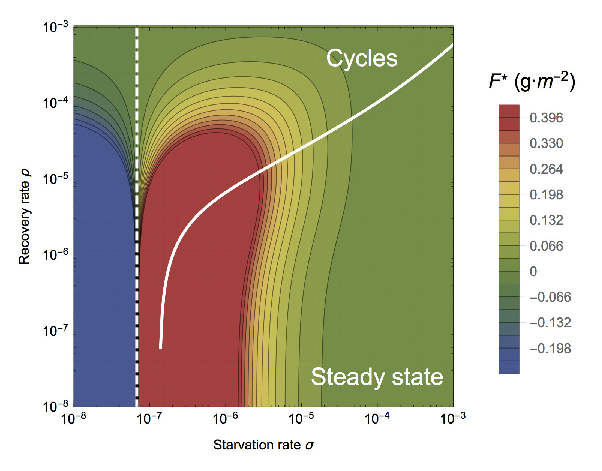
\includegraphics[width=0.4\textwidth]{fig_FixedPoint2.eps}
\caption{\small{ The transcritical (TC; dashed line) and Hopf bifurcation (solid line) as a
  function of the starvation rate $\sigma$ and recovery rate $\rho$ for a 100g consumer.  These
  bifurcation conditions separate parameter space into unphysical (left of the TC), cyclic,
  and steady state dynamic regimes.  The colors show the steady state densities for the energetically replete consumers $F^*$.  
  % Steady state densities for the energetically deficient consumers $H^*$ (not shown)
  % scale with those for $F^*$.  
}\label{fig:fp}}
\end{figure}

Consumers transition from the full state $F$ to the hungry state $H$ at a rate $\sigma$---the starvation rate---and also in proportion to the absence of resources $(1-R)$.  Conversely, consumers recover from state $H$ to state $F$ at rate $\xi \rho$ and in proportion to $R$, where $\xi$ represents a ratio between maximal resource consumption and the carrying capacity of the resource. %and $\approx 2$.
Resources are eaten by the hungry consumers at rate $\rho R + \delta$, that accounts for their somatic growth ($\rho R$) and  maintenance ($\delta$). Full consumers eat resources at a constant rate $\beta$ that accounts for maximal maintenance and somatic growth (see Supplementary Information for mechanistic derivations of these rates from resource energetics).
%This inequality accounts for hungry consumers requiring more resources to replace lost body tissue.
The NSM represents an ecologically motivated fundamental extension of the idealized starving random walk model of foraging, which focuses on resource depletion, to include reproduction and resource replenishment~\citep{Benichou:2014wu,Benichou:2016wl,Chupeau:2016jf}, and is a more general formulation than previous models incorporating starvation~\citep{Persson:1998hz}.

In the mean-field approximation, in which the consumers and resources are perfectly mixed, their densities evolve according to the rate equations

\begin{align}
\label{eq:system}
\begin{split}
\dot{F} &= \lambda F + \xi \rho RH - \sigma \left(1-R\right)F,  \\
\dot{H} &= \sigma \left(1-R\right)F - \xi \rho RH - \mu H,  \\
\dot{R} &= \alpha \left(1-R\right)R -\left(\rho R+\delta\right)H-\beta F
\end{split}
\end{align}

This system of nondimensional equations follows from a set of first-principle relationships for resource consumption and growth (see Supplementary Information for a full derivation and the dimensional form).
Notice that the total consumer density $F+H$ evolves according to $\dot{F}+\dot{H}=\lambda F-\mu H$.
This resembles the equation of motion for the predator density in the classic Lotka-Volterra model~\citep{murray2011mathematical}, except that the resource density does not appear in the growth term.
% As discussed above, the attributes of reproduction and mortality have been explicitly apportioned to the full and hungry consumers, respectively, so that the growth in the total density is decoupled from the resource density.
The rate of reproduction is independent of resource density because it is assumed that the satiated state of the full consumer allows it to partition a constant amount of energy towards reproduction, whereas a starved consumer partitions no energy towards reproduction.
The rate of reproduction for the total consumer density \emph{is} dependent on resource density, which determines the size of the full and starved portions of the consumer population.
Similarly, the consumer maintenance terms ($\delta H$ and $\beta F$) are independent of resource density because they represent a minimal energetic requirement for consumers in the $H$ and $F$ state, respectively.
It follows that model predictions are robust only when $R \gg 0$, which holds for all cases that we explore.


From the solution to the single internal fixed point (Eq.~\eqref{eq:ss}, see Methods), an obvious constraint on the NSM is that the reproduction rate $\lambda$ must be less than the starvation rate $\sigma$, so that the consumer and resource densities are positive.
%In fact, when the resource density $R=0$, the rate equation for $F$ gives exponential growth of $F$ for $\lambda>\sigma$.
The condition $\sigma = \lambda$ thus represents a transcritical (TC) bifurcation~\citep{Strogatz:2008wo} that demarcates a physical from an unphysical regime where all steady-state densities become negative after intersecting the trivial fixed point $(F^*,H^*,R^*)=(0,0,0)$.
The biological implication of the constraint $\lambda<\sigma$ has a simple interpretation---the rate at which a macroscopic organism loses mass due to lack of resources is generally much faster than the rate of reproduction.
As we will discuss below, this inequality is a natural consequence of allometric constraints~\citep{Kempes:2012hy} for organisms within empirically observed body size ranges. %(Fig.~\ref{fig:gvs})

In the physical regime of $\lambda<\sigma$, the fixed point \eqref{eq:ss} may either be a stable node or a limit cycle (Fig.~\ref{fig:fp}).
In continuous-time systems, a limit cycle arises when a pair of complex conjugate eigenvalues crosses the imaginary axis to attain positive real parts~\citep{GuckHolmes}.
This Hopf bifurcation is defined by ${\rm Det}({\bf S}) = 0$, with $\bf S$ the Sylvester matrix, which is composed of the coefficients of the characteristic polynomial of the Jacobian matrix~\citep{Gross:2004p2428}.
As the system parameters are tuned to be within the stable regime, but close to the Hopf bifurcation, the amplitude of the transient cycles becomes large.
Given that ecological systems are constantly being perturbed~\citep{Hastings:2001jh}, the onset of transient cycles, even though they decay with time in the mean-field description, can increase extinction risk~\citep{Neubert:1997wk,Caswell:2005eo,Neubert:2009td}.
%Thus the distance of a system from the Hopf bifurcation provides a measure of its persistence.

When the starvation rate $\sigma\gg\lambda$, a substantial fraction of the consumers are driven to the hungry non-reproducing state.
Because reproduction is inhibited, there is a low steady-state consumer density and a high steady-state resource density.
However, if $\sigma/\lambda\to 1$ from above, the population is overloaded with energetically-replete (reproducing) individuals, thereby promoting transient oscillations between the consumer and resource densities (Fig.~\ref{fig:fp}).
If the starvation rate is low enough that the Hopf bifurcation is crossed, these oscillations become stable over time.
This threshold occurs at higher values of the starvation rate as the recovery rate $\rho$ increases, such that the range of parameter space giving rise to cyclic dynamics also increases with higher recovery rates.

% Whereas the relation between consumer growth rate $\lambda$ and the starvation rate $\sigma$ defines an absolute bound of biological feasibility---the TC bifurcation---$\sigma$ also determines the sensitivity of the consumer population to changes in resource density.
% When $\sigma\gg\lambda$, the steady-state population density is small, thereby increasing the risk of stochastic extinction.
% On the other hand, as $\sigma$ decreases, the system will ultimately be poised either near the TC or the Hopf bifurcation (Fig.~\ref{fig:fp}).
% If the recovery rate $\rho$ is sufficiently small, the TC bifurcation is reached and the resource eventually is eliminated.
% If $\rho$ exceeds a threshold value, cyclic dynamics will develop as the Hopf bifurcation is approached.

\begin{figure}
\centering
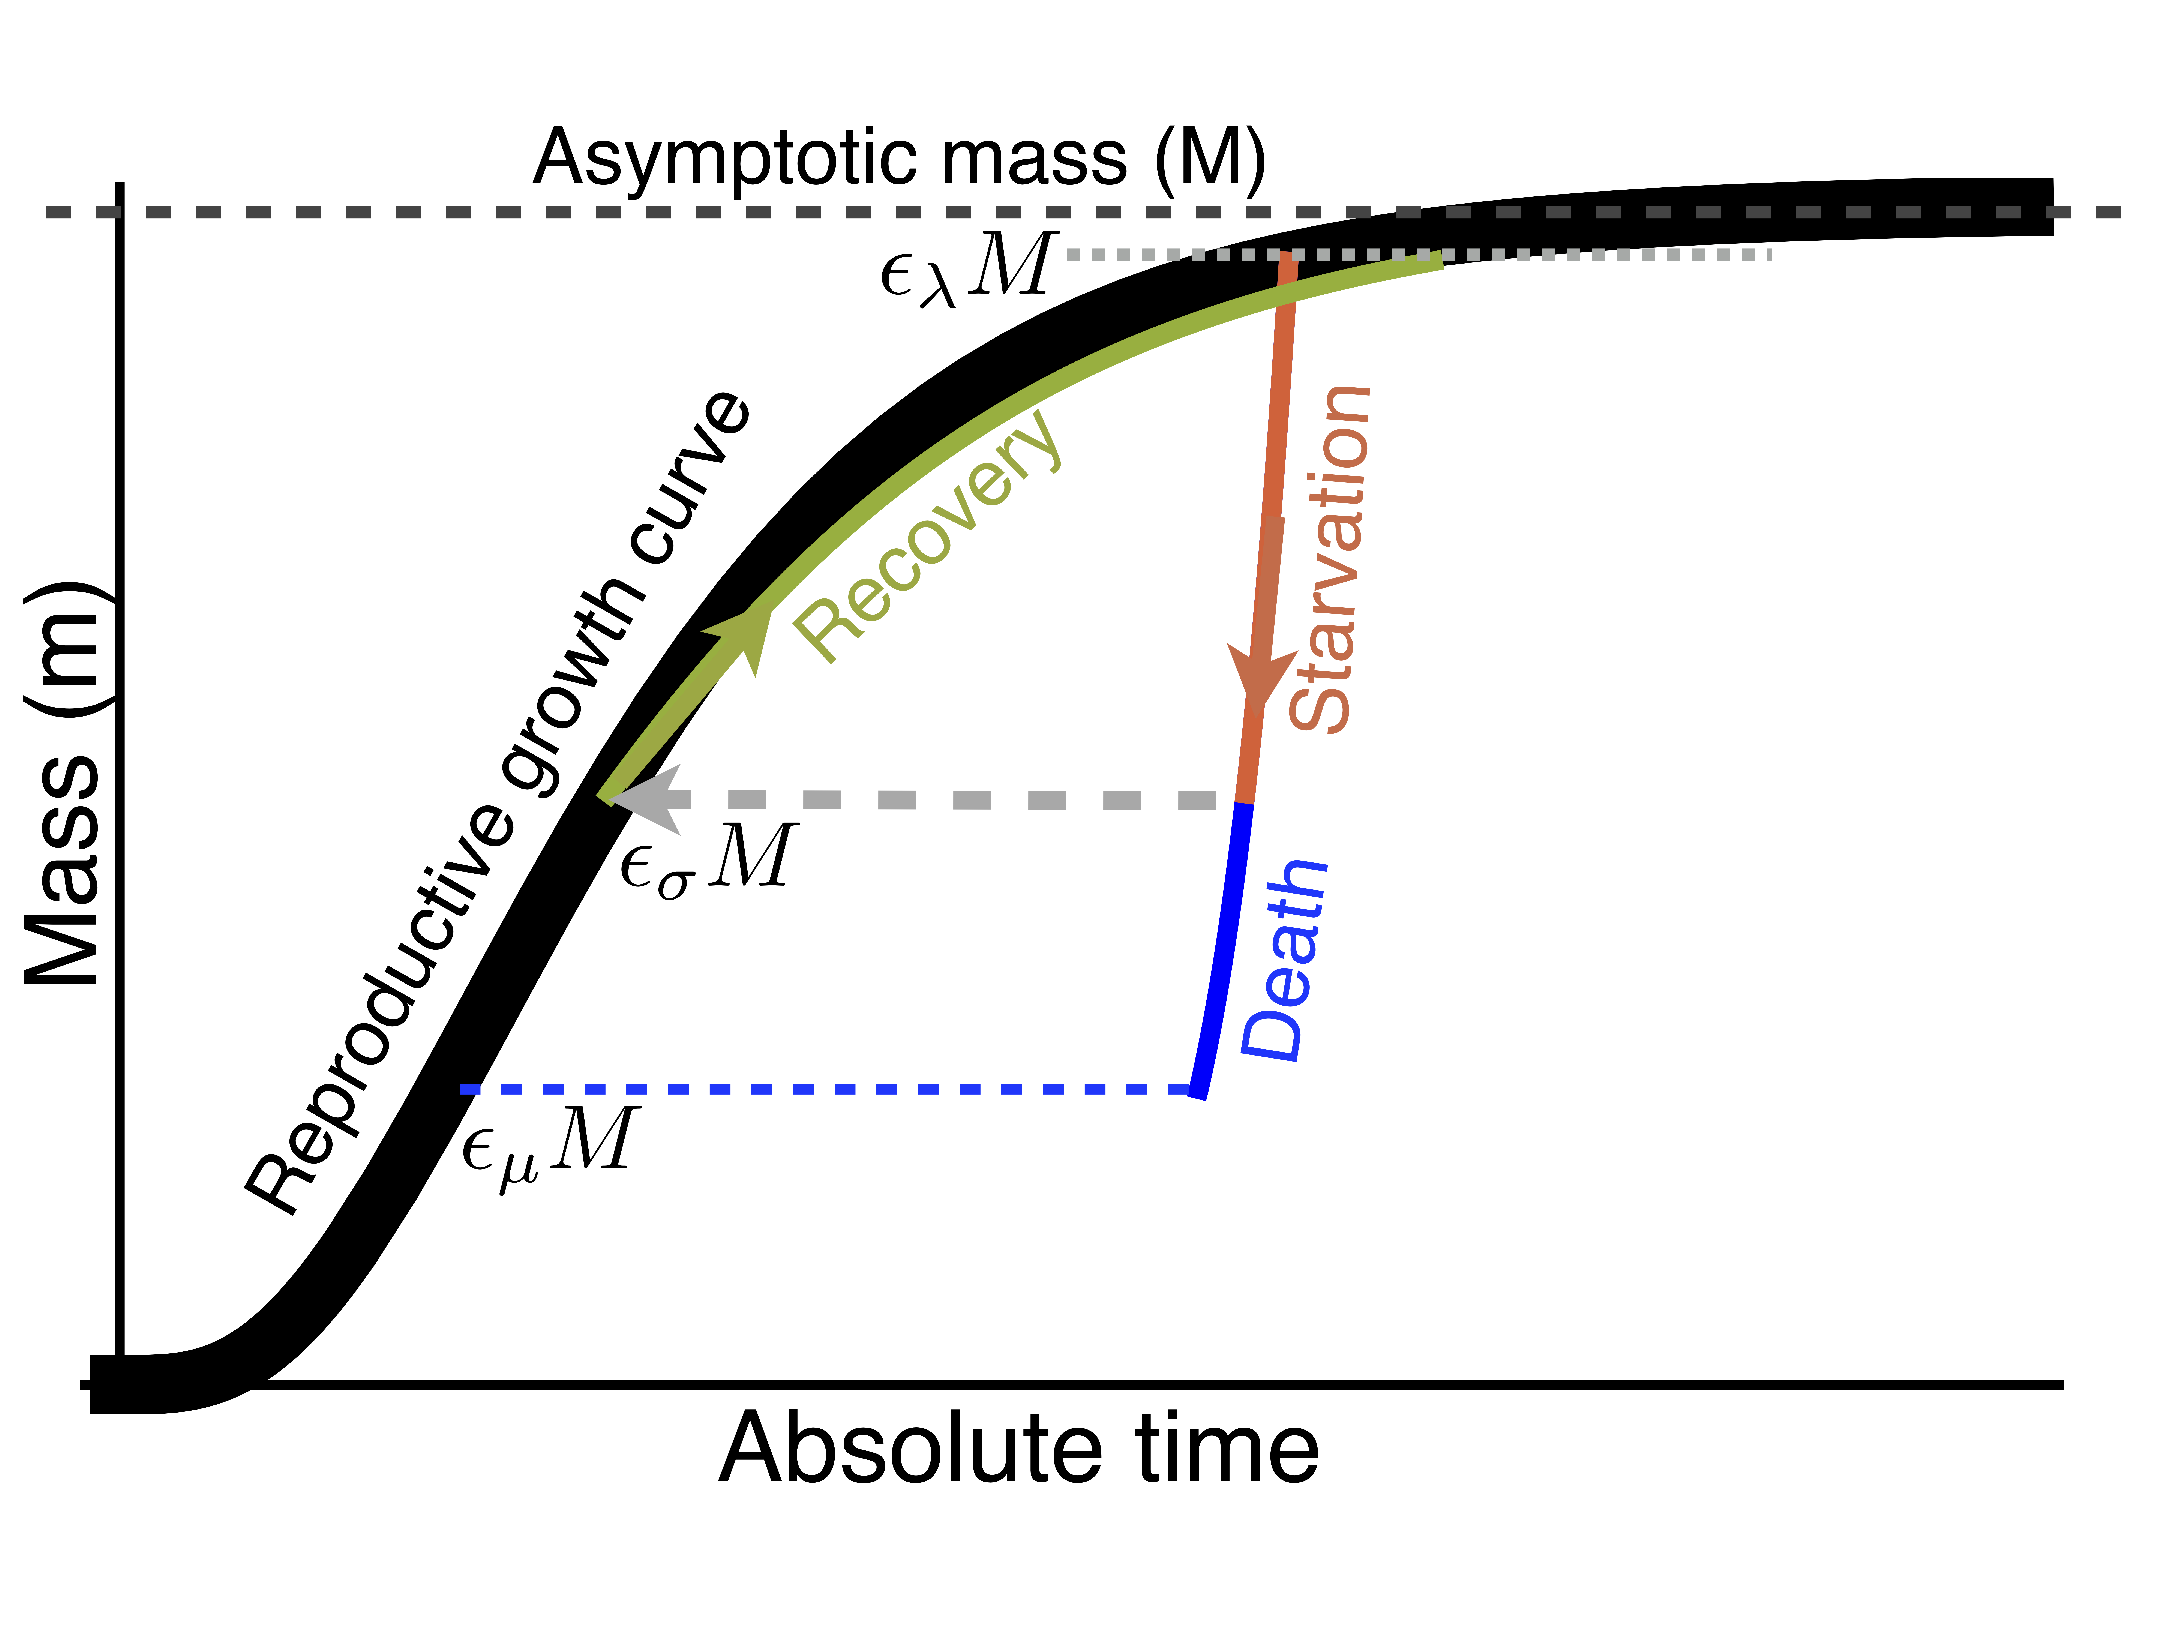
\includegraphics[width=0.4\textwidth]{Growth-trajectory-diagram.eps}
\caption{\small{ The growth trajectory over absolute time of an individual organism as a function of body mass.  
Initial growth follows the black trajectory to an energetically replete reproductive adult mass $m=\epsilon_\lambda M$. %which we assume is 95\% asymptotic mass $M$.  
Starvation follows the red trajectory to $m = \epsilon_\sigma \epsilon_\lambda  M$. 
Recovery follows the green curve to the replete adult mass, where this trajectory differs from the original growth because only fat is being regrown which requires a longer time to reach $\epsilon_\lambda M$. %different energetics and 
Alternatively, death from starvation follows the blue trajectory to $m=\epsilon_\mu \epsilon_\lambda  M$.}\label{fig:growth}}
\end{figure}

% \noindent {\bf Role of allometry} \\
%[Link Allometry stuff to our model - what does it provide to the story]
%[Introduce biological and linked constraints]
%[Allometries capture vast amounts of diversity via a single parameter --- body size]
%[Allometries have captured intterest etc across multiple scales and biological classes of organisms]
While there are no a priori constraints on the parameters in the NSM, most
organisms correspond to restricted portions of the parameter space.  We
use allometric scaling relations to constrain the covariation of rates in a
principled and biologically meaningful manner (see Methods).  Allometric scaling relations
highlight common constraints and average trends across large ranges in body
size and species diversity. Many of these relations can be derived from a
small set of assumptions and in the Methods we describe our framework to determine the
covariation of timescales and rates across a range of body sizes for each of
the key parameters of our model (cf. ref.~\citep{Yodzis:1992hg}).  
% We are thereby able to define the regime of dynamics occupied by the entire class of mammals, along with the key differences between the largest and smallest mammals.

Nearly all of the rates described in the NSM are determined by consumer
metabolism, which can be used to describe a variety of organismal features
\citep{Brown:2004wq}.
We derive relationships for the rates of reproduction, starvation, recovery, and mortality based on first principles, and as a function of an organism's body size and metabolic rate (see Methods).
Because we aim to explore the starvation-recovery dynamics as a function of an organism's body mass $M$, we parameterize these rates in terms of the \emph{percent} gain and loss of the asymptotic (maximum) body mass, $\epsilon M$, where different values of $\epsilon$ defines different states of the consumer (Fig.~\ref{fig:growth}).
Although the rate equations \eqref{eq:system} are general and can in principle be used to explore the starvation recovery dynamics for most organisms, here we focus on allometric relationships for terrestrial-bound lower trophic level endotherms (see Supplementary Information for values), specifically herbivorous mammals, which range from a minimum of $M\approx1$g (the Etruscan shrew \emph{Suncus etruscus}) to a maximum of $M\approx10^7$g (the early Oligocene Indricotheriinae and the Miocene Deinotheriinae).
Investigating other classes of organisms would simply involve altering the metabolic exponents and scalings associate with $\epsilon$. Moreover, we emphasize that our allometric equations describe mean relationships, and do not account for the (sometimes considerable) variance associated with individual species.\\

% \noindent {\bf  Stabilizing effects of allometric constraints} \\
% As the allometric derivations of the NSM rate laws reveal, starvation and recovery rates are not independent parameters, and the biologically relevant portion of the phase space shown in Fig.~\ref{fig:fp} is constrained via covarying parameters.
% Given the parameters of terrestrial endotherms, we find that the starvation rate $\sigma$ and the recovery rate $\rho$ are constrained to lie within a small region of potential values for the known range of body sizes $M$.
% Moreover, the dynamics for all mammalian body sizes are confined to the steady-state regime of the NSM and that limit-cycle behavior is precluded.
%Incorporating uncertainty in allometric parameters (20\% variation around the mean; Fig.~\ref{fig:hopf}), we find that, for larger $M$, the distance to the TC and Hopf bifurcation decreases.
% These results suggest that small mammals are marginally less prone to population oscillations---both stable limit cycles and transient cycles---than mammals with larger body size.  However, starvation and recovery rates across all values of $M$ fall squarely in the steady state region at some distance from the Hopf bifurcation. 
% This result suggests that cyclic population dynamics should be rare, particularly in environments where resources are limiting.\\


% Previous studies used allometric constraints to explain the periodicity of cyclic populations \citep{CalderIII:1983jd,Peterson:1984hj,Krukonis:1991fk}, suggesting a period $\propto M^{0.25}$.
% However this relation seems to hold only for some species \citep{Hendriks:2012fc}, and potential drivers of variation and systematically different behavior range from predator and/or prey lifespans to competitive dynamics~\citep{Kendall:1999iy,Hogstedt:2005cr}.
% Statistically significant support for the existence of population cycles among mammals is relatively rare, though predominantly based on time series for small mammals~\citep{Kendall:1998hl}.
% However the longer gestational times and increased difficulty in collecting adequate data precludes obtaining similar-quality information for larger organisms.\\ 



\begin{figure*}
\centering
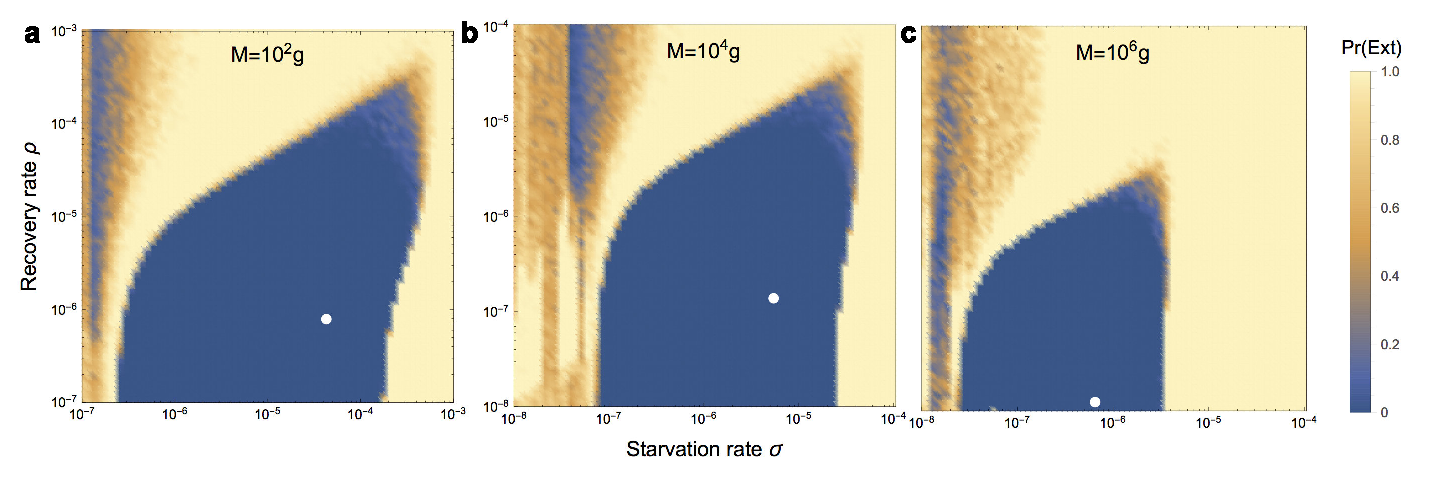
\includegraphics[width=0.8\textwidth]{fig_ExtinctionAllometricComb3.eps}
\caption{\small{ Probability of extinction for a consumer with ({\bf a}) $M=10^2$g, ({\bf b}) $M=10^4$g, and ({\bf c}) $M=10^6$g as a function of the starvation rate $\sigma$ and recovery rate $\rho$, where the initial density is given as $(XF^*,XH^*,R^*)$, where $X$ is a random uniform variable in $[0,2]$. Note the change in scale for $M=10^4$ and $M=10^6$g.  Extinction is defined as the population trajectory falling below $0.2\times$ the allometrically constrained steady state. The white points denote the allometrically constrained starvation and recovery rate.}\label{fig:ext}}
\end{figure*}

%Extinction to the left and the right
\noindent {\bf Extinction risk}\\
As the allometric derivations of the NSM rate laws reveal (see Methods), starvation and recovery rates are not independent parameters, and the biologically relevant portion of the phase space shown in Fig.~\ref{fig:fp} is constrained via covarying parameters.
Given the parameters of terrestrial endotherms, we find that the starvation rate $\sigma$ and the recovery rate $\rho$ are constrained to lie within a small region of potential values for the known range of body sizes $M$.
Indeed, starvation and recovery rates across all values of $M$ fall squarely in the steady state region at some distance from the Hopf bifurcation. 
This suggests that cyclic population dynamics should be rare, particularly in environments where resources are limiting.
% Moreover, the dynamics for all mammalian body sizes are confined to the steady-state regime of the NSM and that limit-cycle behavior is precluded.

Higher rates of starvation result in a larger flux of the population to the hungry state.
In this state, reproduction is absent, thus increasing the likelihood of extinction.  From the perspective of population survival, it is the rate of starvation relative to the rate of recovery that determines the long-term dynamics of the various species (Fig.~\ref{fig:fp}).
We therefore examine the competing effects of cyclic dynamics vs. changes in steady-state density on extinction risk, both as functions of $\sigma$ and $\rho$.
To this end, we computed the probability of extinction, where we define extinction as a population trajectory falling below one fifth of the allometrically constrained steady state at any time between $t=10^8$ and $t=10^{10}$.
This procedure is repeated for 50 replicates of the continuous-time system shown in Eq.~\ref{eq:system} for organisms with mass ranging from $10^2$ to $10^6$ grams.
%the initial condition isdistributed around the steady state (Eq.~\ref{eq:ss}).  Specifically
In each replicate the initial densities are chosen to be $(XF^*,XH^*,R^*)$, with $X$ a random variable that is uniformly distributed in $[0,2]$.
By allowing the rate of starvation to vary, we assessed extinction risk across a range of values for $\sigma$ and $\rho$ between ca.\ $10^{-7}$ to $10^{-3}$. %, thus examining a horizontal cross-section of Fig.~\ref{fig:fp}.
As expected, higher rates of extinction correlate with both high values of $\sigma$ if $\rho$ is small, and high values of $\rho$ if $\sigma$ is small.
For low values of $\sigma$ and high values of $\rho$, the increased extinction risk results from transient cycles with larger amplitudes as the system nears the Hopf bifurcation (Fig.~\ref{fig:ext}).
For high values of $\sigma$ and low values of $\rho$, increased extinction risk arises because of the decrease in the steady-state consumer population density (Figs. \ref{fig:fp}b, \ref{fig:ext}).
This interplay creates an `extinction refuge', such that for a constrained range of $\sigma$ and $\rho$, extinction probabilities are minimized.

We find that the allometrically constrained values of $\sigma$ and $\rho$ fall squarely within the extinction refuge across a range of $M$ (Fig. \ref{fig:ext}a-c, white points).
These values are close enough to the Hopf bifurcation to avoid low steady-state densities, and far enough away to avoid large-amplitude transient cycles.
The feature that allometric values of $\sigma$ and $\rho$ fall within this relatively small window supports the possibility that a selective mechanism has constrained the physiological conditions that drive starvation and recovery rates within populations.
Such a mechanism would select for organism physiology that generates appropriate $\sigma$ and $\rho$ values that serve to minimize extinction risk.
This selection could occur via the tuning of body fat percentages, metabolic rates, and biomass maintenance efficiencies.
We also find that as body size increases, the amount of low extinction risk parameter space becomes smaller (Fig. \ref{fig:ext}a-c), suggesting that the population dynamics of larger organisms are more sensitive to smaller changes in physiological rates controlling starvation and recovery.
% OLD WORDING Such a mechanism would involve a feedback between the dynamics of the population and the fitness of individuals within the population, though to what extent the dynamics of the population influence rates of starvation and recovery would also involve potential tradeoffs in reproduction and somatic maintenance.
To summarize, our finding that the allometrically-determined parameters fall within this low extinction probability region suggests that the NSM dynamics may both drive---and constrain---natural animal populations.\\



%Results are insensitive to alpha but possibly sensitive to beta (eff parameter)


%NOTES 7/8/16
%Calder has a hypothesis that period ~ Mass^(1/4).
%Can we get "transient period" from Jacobian?
%Lots of food web lit on stabilizing effects of body size! Brose, Petchey for instance. Good for discussion.

\noindent {\bf Discussion}\\
Metabolite transport constraints are widely thought to place strict boundaries on biological scaling~\citep{Brown:1993p708,West:1997cg,Brown:2004wq} and thereby lead to specific predictions on the minimum possible body size for organisms~\citep{West:2002ud}.
Above this bound, a number of energetic and evolutionary mechanisms have been explored to assess the costs and benefits associated with larger body masses, particularly for mammals.
One important such example is the \emph{fasting endurance hypothesis}, which contends that larger body size, with consequent lower metabolic rates and increased ability to maintain more endogenous energetic reserves, may buffer organisms against environmental fluctuations in resource availability~\citep{Millar:1990p923}.
Over evolutionary time, terrestrial mammalian lineages show a significant trend towards larger body size (known as Cope's rule)~\citep{Alroy:1998p1594,Clauset:2009fh,Smith:2010p3442,Saarinen:2014br}, and it is thought that within-lineage drivers generate selection towards an optimal upper bound of roughly $10^7$ grams~\citep{Alroy:1998p1594}, a value that is likely limited by higher extinction risk for large taxa over longer timescales~\citep{Clauset:2009fh}.
These trends are thought to be driven by a combination of climate change and niche availability~\citep{Saarinen:2014br}; however the underpinning energetic costs and benefits of larger body sizes, and how they influence dynamics over ecological timescales, have not been explored.
We argue that the NSM provides a suitable framework to explore these issues.



\noindent {\bf Energetic barriers to body size}
The NSM correctly predicts that species with smaller masses have larger steady-state population densities (Fig.~\ref{fig:mass}a).
Similar predictions have been made for carnivore populations using alternative consumer-resource models \citep{DeLong:2012kw}.
Moreover, we show that the NSM provides independent theoretical support for the energy equivalence hypothesis and Damuth's Law \citep{Damuth:1987kr,allen2002,enquist1998}.
The energy equivalence hypothesis argues that the total energy use, $B_{\rm tot}$, of a population is constant independent of species size~\citep{Damuth:1987kr,allen2002,enquist1998}. %Previous studies have focused on t
This hypothesis is based on observations showing that the steady state abundance, $N^*$, of a species is proportional to the inverse of individual metabolism, such that $N^*\propto M^{-3/4}/B_{0}$~\citep{allen2002,enquist1998}.
This relationship implies that $B_{\rm tot}=N^*B(M)=Q$, where $Q$ is a constant, and has been shown to hold in both mammalian and vascular plant communities \citep{Damuth:1987kr,allen2002,enquist1998}.
Figure \ref{fig:mass}a shows that both $F^{*}$ and $H^{*}$ scale as $M^{-\eta}$ over a wide range of organism sizes and Figure \ref{fig:mass}b shows that $F^{*}B$ is nearly constant over this same range.
This result is remarkable because it illustrates that the steady state values of the NSM combined with the derived timescales naturally give rise to energy equivalence.


\begin{figure}
\centering
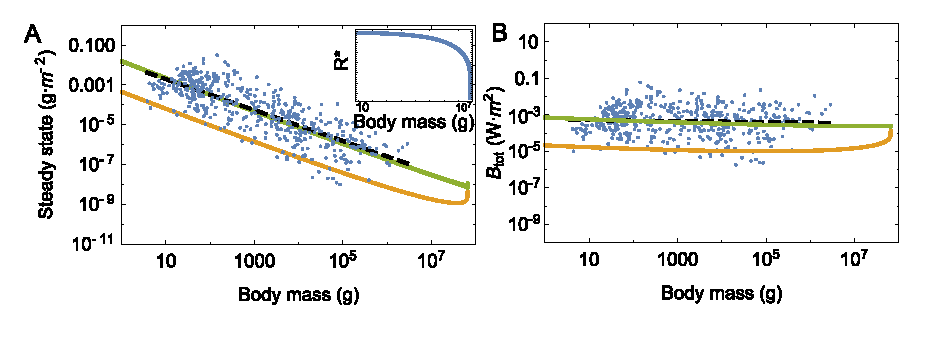
\includegraphics[width=0.48\textwidth]{fig_FPAllometric2.eps}
\caption{\small{ ({\bf a}) Consumer steady states $F^*$ (green) and $H^*$ (orange) as a function of
  body mass. Inset: Resource steady state $R^*$ as a function of consumer body mass.
  ({\bf b}) Total energetic use $B_{\rm tot}$ of consumer populations at the steady state as a function of body mass.
  The data are from Damuth \citep{Damuth:1987kr} and have been converted to total population metabolism using the allometric relationships for metabolic rate (please see Supplementary Information and Refs. \citep{West:2001bv,hou,moses2008rmo}).}\label{fig:mass}}
\end{figure}

Our model shows that the equivalence breaks down at large $M$ suggesting that this maximum is a hard limit where deviations outside of this range are energetically suboptimal. %, violating the energy equivalence. % set by deviations from constant efficiency obeyed by other populations.
In the framework of our model, the total metabolic rate of $F$ and $H$ becomes infinite at a finite mass, and occur at the same scale where the steady state resources vanish (Fig.~\ref{fig:mass}). This asymptotic behavior is governed by body sizes at which $\epsilon_{\mu}$ and $\epsilon_{\lambda}$ equal zero, causing the timescales to become infinite and the rates $\mu$ and $\lambda$ to equal zero.
The $\mu=0$ asymptote occurs first when $f_{0}M^{\gamma-1}+u_{0}M^{\zeta-1}=1$, and corresponds to $(F^*,H^*,R^*)=(0,0,0)$. This point predicts a strong upper bound on mammalian body size and occurs at $M_{\rm max}=6.54\times10^7$.
Moreover, $M_{\rm max}$, which is entirely determined by the population-level consequences of energetic constraints, is within an order of magnitude of the maximum body size observed in the North American mammalian fossil record~\citep{Alroy:1998p1594}, as well as the mass predicted from an evolutionary model of body size evolution~\citep{Clauset:2009fh}.
It should be noted that the asymptotic behavior and predicted upper bound depend only on the scaling of body composition and are independent of the resource parameters.
We also note that the prediction of an asymptotic limit on mammalian size parallels work on microbial life where an upper and lower bound on bacterial size, and an upper bound on single cell eukaryotic size, is predicted from similar growth and energetic scaling relationships~\citep{Kempes:2012hy,Kempes:2016}. % reasons or from dissimilar scaling of cellular composition which is analogous to the body fat composition employed here
\\

%Significant deviations from constant energy use occur at $M \lesssim 1$ at the small end of the mammalian range and $M\approx 6.5*10^7$ at the large end.
%Compellingly, this dynamic bound, which is determined by the rate of energetic recovery, is close to the minimum observed mammalian body size of ca.\ 1.3-2.5g, a range that occurs as the recovery rate begins its decline.
%In addition to known transport limitations~\citep{West:2002ud}, we suggest that an additional constraint of lower body size stems from the dynamics of starvation.
%This result mirrors other efforts \citep{Kempes:2012hy,Kempes:2016} where at a given scale multiple limitations constrain the smallest possibilities for life within a class of organisms.

%The combined steady-state dynamics and allometric timescales of the NSM predict that larger mammals should outcompete smaller ones, and this suggests that the model may provide a framework with which to explore the energetic mechanisms behind Cope's rule. %, which we explore further below.

\noindent{\bf A within-lineage driver of Cope's Rule}
The NSM predicts that the steady state resource density $R^{*}$ decreases with increasing body size of the consumer population (Fig. \ref{fig:mass}a, inset), and classic resource competition theory predicts that the species surviving on the lowest resource abundance will outcompete others \citep{tilman1981,dutkiewicz2009,barton2010}. Thus, the combined NSM steady-state dynamics and allometric timescales predict that larger mammals have an intrinsic competitive advantage given a common resource, but these absolute limits do not offer a within-lineage mechanism by which larger body sizes are selected for or against.
We will now show that the NSM indeed provides a mechanistic understanding of the energetic dynamics that give rise to both observed limitations on mammalian body size, as well as the observed trend towards larger body size over evolutionary time known as Cope's Rule.

\begin{figure}
\centering
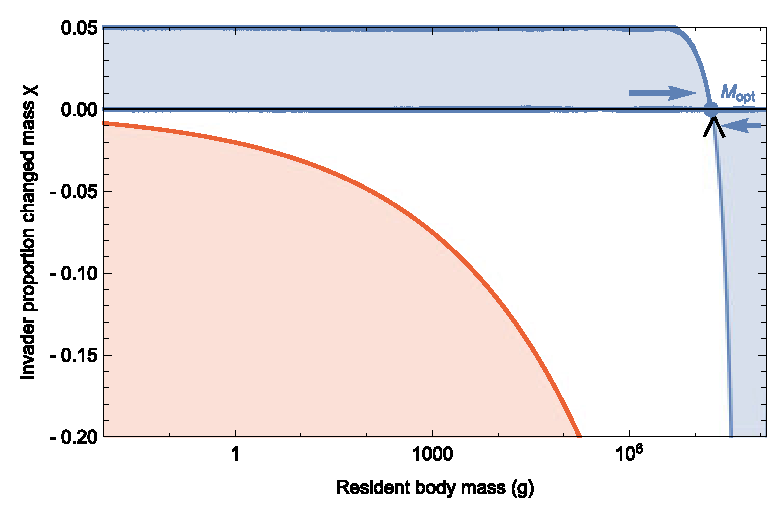
\includegraphics[width=0.4\textwidth]{fig_Invasion.eps}
\caption{\small{ Invasion feasibility for organisms with a proportional change in
  mass $\chi$ against a population with a resident body mass $M$.  The blue
  region denotes proportions of modified mass $\chi$ resulting in successful invasion.  The
  red region denotes values of $\chi$ that result in a mass that is below the
  starvation threshold and are thus infeasible.
  Arrows point to the predicted optimal mass from our model $M_{\rm opt}=1.748\times 10^7$, which may serve as an evolutionary attractor for body mass.
  The black wedge points to the largest body mass known for terrestrial mammals (\emph{Deinotherium} spp.) at $1.74\times10^7$g~\citep{Smith:2010p3442}.}\label{fig:invasion}}
\end{figure}


To examine whether the NSM could provide such a mechanism, we begin by noting that a theoretical upper bound on mammalian body size is given by $\epsilon_\sigma=0$, where mammals are entirely composed of metabolic reserves, and this occurs at $M=8.3\times 10^8$, or $120$ times the mass of a male African elephant.
Next we examine to what extent a more realistic upper bound to body mass may serve as an evolutionary attractor, thus providing a suitable within-lineage mechanism for Cope's rule.

We directly assess the susceptibility of an otherwise homogeneous population to invasion by a mutated subset of the population (denoted by $^\prime$) where individuals have a modified proportion of body fat $M^\prime=M(1+\chi)$.
If $\chi < 0$, individuals within the invading mutant population have fewer metabolic reserves, and if $\chi>0$, individuals have more metabolic reserves than the resident population.
For the allowable values of $\chi$ the adjusted mass should exceed the minimal amount of body fat, $1+\chi>\epsilon_{\sigma}$, and the adjusted time to reproduce must be positive, which given Equation \ref{t1}, implies that $1-\epsilon_{\lambda}^{1-\eta}\left(1+\chi\right)^{1-\eta}>0$.
Together these conditions imply that  $\chi\in(-f_0M^{\gamma-1},1/\epsilon_{\lambda}-1)$ where the upper bound approximately equals $0.05$ and the lower bound is mass-dependent.
The modified mass adjusts our model via the altered rates of starvation $\sigma(M^\prime)$, recovery $\rho(M^\prime)$, and the maintenance of both starving $\delta(M^\prime)$ and full consumers $\beta(M^\prime)$.
Importantly, $\epsilon_\sigma$, which determines the point along the growth curve that defines the body composition of starved foragers, is assumed to remain unchanged for the invader population (see Supplementary Information for detailed derivations of invader rates).
%There is no internal fixed point corresponding to a state where both original residents and invaders coexist (except for the trivial state $\chi=0$).

To assess the susceptibility of the resident population to invasion, we determine which consumer pushes the steady-state resource density to lower values for a given value of $\chi$, with the expectation that populations able to survive on lower resource densities have a competitive advantage \citep{tilman1981}.
We find that for $M\leq 1.748\times10^7$g, having additional body fat ($\chi > 0$) results in a lower steady state resource density ($R^{\prime *}<R^*$), such that the invader has an intrinsic competitive advantage over the resident population (Fig. \ref{fig:invasion}).
However, for $M> 1.748\times10^7$g, leaner individuals ($\chi < 0$) have lower resource steady state densities, switching the advantage from having more metabolic reserves to having less.

%, and this is due to the changing
%covariance between energetic rates as a function of modified energetic
%reserves \sid{I don't understand the phrase after the comma AND STILL DON'T}.



The observed switch in susceptibility as a function of $\chi$ at $M_{\rm opt}= 1.748\times10^7$g thus serves as an attractor, such that the NSM predicts organismal mass to increase if $M<M_{\rm opt}$ and decrease if $M>M_{\rm opt}$.
This value is close to but smaller than the asymptotic upper bound for terrestrial mammal body size predicted by the NSM, however it is remarkably close to independent estimates of the largest land mammals, the early Oligocene \emph{Indricotherium} at ca. $1.5\times10^7$g and the late Miocene \emph{Deinotherium} at ca. $1.74\times10^7$g ~\citep{Smith:2010p3442}.
Additionally, our calculation of $M_{\rm opt}$ as a function of mass-dependent physiological rates is similar to theoretical estimates of maximum body size \citep{Clauset:2009fh}, and provides independent theoretical support for the observation of a `maximum body size attractor' for North American mammals outlined by Alroy~\citep{Alroy:1998p1594}.
%as well as  \citep{Alroy:1998p1594,Clauset:2009fh}.
%This value is only XX\% the estimated size of Indricotheriinae, a group that includes the largest known terrestrial mammal.
While the state of the environment, as well as the competitive landscape, will determine whether specific body sizes are selected for or against~\citep{Saarinen:2014br}, we propose that the dynamics of starvation and recovery described in the NSM provide a general within-lineage mechanism for the evolution of larger body size among terrestrial mammals.


%and we suggest that the starvation dynamics described here act in concert with these other factors is the only driver of body size evolution.


%One might be concerned a greater number of large mammals are currently not observed in the modern world given that larger mammals are less susceptible to extinction.
%However, recent research suggests that the pleistocene may have been much more populated with a significant diversity of very large mammals \citep{Doughty:2013kd,Doughty:2015hy,Doughty:2015je} which were also much more geographically widespread than today.
%These results, combined with our findings, suggest that the modern diversity of mammals may not represent a true steady state the current distribution of nutrients and large seeds may be very different from the past \citep{Doughty:2013kd,Doughty:2015hy,Doughty:2015je}.

%Closing
The energetics associated with somatic maintenance, growth, and reproduction are important elements that influence the dynamics of all populations~\citep{Stearns:1989ip}.
The NSM is a minimal and general model that incorporates the dynamics of starvation and recovery that are expected to occur in resource-limited environments.
By incorporating allometric relations between the rates in the NSM, we found: (i) different organismal masses have distinct population dynamic regimes, (ii) allometrically-determined rates of starvation and recovery appear to minimize extinction risk, and (iii) the dynamic consequences of these rates may introduce additional drivers and hard boundaries on the evolution of maximum body size.
We suggest that the NSM offers a means by which the dynamic consequences of energetic constraints can be assessed using macroscale interactions between and among species.
Future efforts will involve exploring the consequences of these dynamics in a spatially explicit framework, thus incorporating elements such as movement costs and spatial heterogeneity, which may elucidate additional tradeoffs associated with the dynamics of starvation and recovery.



\section*{Methods}
\small{
{\bf Analytical solution to the NSM}
Equation~\eqref{eq:system} has three fixed points: two trivial fixed points at $(F^*,H^*,R^*)=(0,0,0)$ and $(0,0,1)$, and one non-trivial, internal fixed point at
\begin{align}
\label{eq:ss}
\begin{split}
F^* &= (\sigma-\lambda)\frac{ \alpha  \lambda  \mu ^2  (\mu +\xi  \rho )}{A (\lambda  \rho  B+\mu  \sigma  (\beta  \mu +\lambda  (\delta +\rho )))}, \\
H^* &= (\sigma-\lambda)\frac{ \alpha  \lambda ^2 \mu  (\mu +\xi  \rho )}{A (\lambda  \rho  B+\mu  \sigma  (\beta  \mu +\lambda  (\delta +\rho )))}, \\
R^* &= (\sigma - \lambda)\frac{\mu  }{A}.
\end{split}
\end{align}
where $A=(\lambda  \xi  \rho +\mu  \sigma )$ and $B=(\beta  \mu  \xi +\delta  \lambda  \xi -\lambda  \mu )$. The stability of this fixed point is determined by the Jacobian matrix $\bf J$, where each matrix element $J_{ij}=\partial{\dot X_i}/\partial{X_j}$ when evaluated at the internal fixed point, and $\mathbf{X}$ is the vector $(F,H,R)$.
The parameters in Eq.~\eqref{eq:system} are such that the real part of the largest eigenvalue of $\mathbf{J}$ is negative, so that the system is stable with respect to small perturbations from the fixed point.
Because this fixed point is unique, it is the global attractor for all population trajectories for any initial condition where the resource and consumer densities are both nonzero.

{\bf Metabolic scaling relationships}
The scaling relation between an organism's metabolic
rate $B$ and its body mass $M$ at reproductive maturity is known to scale as
$B = B_0 M^\eta$~\citep{West:2002it}, where the scaling exponent $\eta$ is
typically close to $2/3$ or $3/4$ for metazoans (e.g., ref. \citep{Brown:2004wq}),
and has taxonomic shifts for unicellular species between $\eta\approx 1$ in
eukaryotes and $\eta\approx 1.76$ in bacteria
\citep{DeLong:2010dy,Kempes:2012hy}.
%Justin adding an explanation for beta

Several efforts have shown how a partitioning of $B$ between growth and
maintenance purposes can be used to derive a general equation for both the
growth trajectories and growth rates of organisms ranging from bacteria to
metazoans
\citep{West:2001bv,moses2008rmo,gillooly2002esa,hou,Kempes:2012hy}. This relation is derived from the simple balance condition 
$B_{0}m^{\eta}=E_{m}\dot{m}+B_{m}m\,,$
% \begin{eqnarray}
% \label{balance}
% B_{0}m^{\eta}=E_{m}\frac{dm}{dt}+B_{m}m\,,
% \end{eqnarray}
\citep{West:2001bv,moses2008rmo,gillooly2002esa,hou,Kempes:2012hy} where $E_{m}$ is the energy needed to synthesize a unit of mass, $B_{m}$ is
the metabolic rate to support an existing unit of mass, and $m$ is the mass
of the organism at any point in its development.  This balance has the
general solution \citep{bettencourt,Kempes:2012hy}
\begin{eqnarray}
\label{m1}
\left(\frac{m\left(t\right)}{M}\right)^{1-\eta}\!=1\!-\!\left[1\!-\!\left(\frac{m_{0}}{M}\right)^{1\!-\!\eta}\right]e^{-a\left(1\!-\!\eta\right)t/M^{1-\eta}},
\end{eqnarray}
where, for $\eta<1$, $M=(B_{0}/B_{m})^{1/(1-\eta)}$ is the asymptotic mass, $a=B_{0}/E_{m}$, and $m_0$ is mass at birth, itself varying allometrically (see Supplementary Information).  We now use this solution to define the timescale for reproduction and recovery from starvation (Fig.~\ref{fig:growth}; see \citep{moses2008rmo} for a detailed presentation of these timescales). The time that it takes to reach a particular mass $\epsilon M$ is given by the timescale
\begin{equation}
\label{t1}
\tau\left(\epsilon\right) = \ln\left[\frac{1-\left(m_{0}/M\right)^{1-\eta}}{1-\epsilon^{1-\eta}}\right]\frac{M^{1-\eta}}{a\left(1-\eta\right)},
\end{equation}
where we will define values of $\epsilon$ to describe a set of rates within our model. For the time to reproduce, $t_{\lambda}=\tau\left(\epsilon_{\lambda}\right)$, where $\epsilon_{\lambda}$ is the fraction of the asymptotic mass where an organism is reproductively mature and should be close to one (typically $\epsilon_{\lambda}\approx0.95$; \citep{West:2001bv}). The growth rate is then given by $\lambda=\ln\left(\upsilon\right)/t_{\lambda}$ where $\upsilon$ is the number of offspring produced, and for any constant value of $\epsilon_{\lambda}$, this rate will scale as $\lambda\propto M^{\eta-1}$ for $M\gg m_{0}$ \citep{West:2001bv,moses2008rmo,gillooly2002esa,hou,Kempes:2012hy}.


The rate of recovery $\rho = 1/t_\rho$ requires that an organism accrues
sufficient tissue to transition from the hungry to the full state.  Since
only certain tissues can be digested for energy (for example the brain cannot
be degraded to fuel metabolism), we define the rates for starvation, death,
and recovery by the timescales required to reach, or return from, specific
fractions of the replete-state mass (see Supplementary Information, Table I for parameterizations).  We define
$m_{\sigma}=\epsilon_{\sigma} M$, where $\epsilon_{\sigma}<1$ is the fraction of
replete-state mass where reproduction ceases. This fraction will deviate from a constant
if tissue composition systematically scales with adult mass.  For example,
making use of the observation that body fat in mammals scales with overall
body size according to $M_{\rm fat}=f_{0}M^{\gamma}$ and assuming that once
this mass is fully digested the organism starves, this would imply that
$\epsilon_{\sigma}=1-f_{0}M^{\gamma}/M$. It follows that the
recovery timescale, $t_{\rho}$, is the time to go from
$m=\epsilon_{\sigma} \epsilon_{\lambda} M$ to $m=\epsilon_{\lambda}M$ (Fig. \ref{fig:growth}). Using Eqs.~\eqref{m1} and \eqref{t1} this timescale is given by simply considering an adjusted starting mass of $m_{0}^{\prime}=\epsilon_{\sigma}\epsilon_{\lambda}M$, in which case
\begin{eqnarray}
\label{rhotimescale}
t_{\rho}=\ln\left[\frac{1-\left(\epsilon_{\sigma}\epsilon_{\lambda}\right)^{1-\eta}}{1-\epsilon_\lambda^{1-\eta}}\right]\frac{M^{1-\eta}}{a^{\prime}\left(1-\eta\right)}
\end{eqnarray}
where $a^{\prime}=B_{0}/E_{m}^{\prime}$ accounts for possible deviations in the biosynthetic energetics during recovery (see Supplementary Information). It should be noted that more complicated ontogenetic models explicitly handle
storage \citep{hou}, whereas this feature is implicitly covered by the body
fat scaling in our framework.



To determine the starvation rate, $\sigma$, we are interested in the time
required for an organism to go from a mature adult that reproduces at rate
$\lambda$, to a
reduced-mass hungry state where reproduction is impossible.  For starving individuals we assume that an organism must meet its maintenance requirements by using the digestion of existing mass as the sole energy source.
This assumption implies the following simple metabolic balance
$\dot{m}E_{m}^{\prime}=-B_{m}m$ or $\dot{m}=-a^{\prime}m/M^{1-\eta}$
% \begin{eqnarray}
% \frac{dm}{dt}E_{m}^{\prime}=-B_{m}m
% \end{eqnarray}
% or
% \begin{eqnarray}
% \frac{dm}{dt}=-\frac{a^{\prime}}{M^{1-\eta}}m
% \end{eqnarray}
where $E_{m}^{\prime}$ is the amount of energy stored in a unit of existing
body mass, which differs from $E_{m}$, the energy required to
synthesis a unit of biomass \citep{hou}. Given the replete mass, $M$, of an organism, the
above energy balance prescribes the mass trajectory of a non-consuming
organism:$m\left(t\right)=Me^{-a^{\prime}t/M^{1-\eta}}$.
% \begin{eqnarray}
% \label{mt}
% m\left(t\right)=Me^{-a^{\prime}t/M^{1-\eta}}.
% \end{eqnarray}
The timescale for starvation is
given by the time it takes $m(t)$ to reach $\epsilon_{\sigma} M$, which gives
\begin{equation}
\label{eq:sigma}
t_{\sigma}=-\frac{M^{1-\eta}}{a^{\prime}}\ln\left(\epsilon_{\sigma}\right).
\end{equation}
The starvation rate is then $\sigma=1/t_{\sigma}$, which scales with
replete-state mass as $1/M^{1-\eta}\ln\left(1-f_{0}M^{\gamma}/M\right)$.  An important
feature is that $\sigma$ does not have a simple scaling dependence on
$\lambda$, which is important for the dynamics that we
later discuss.

The time to death should follow a similar relation, but defined by a lower
fraction of replete-state mass, $m_{\mu}=\epsilon_{\mu} M$ where $\epsilon_\mu < \epsilon_\sigma$.
Suppose, for example, that an organism dies once it has digested all fat and
muscle tissues, and that muscle tissue scales with body mass according to
$M_{\rm musc}=u_{0}M^{\zeta}$.  This gives
$\epsilon_{\mu}=1-\left(f_{0}M^{\gamma}+u_{0}M^{\zeta}\right)/M$. Muscle
mass has been shown to be roughly proportional to body mass~\citep{Folland:2008ij} in
mammals and thus $\epsilon_{\mu}$ is merely $\epsilon_{\sigma}$ minus a constant. The time to go from starvation to death is the total time to reach $\epsilon_{\mu}M$ minus the time to starve, or $t_{\mu}=-M^{1-\eta}\ln\left(\epsilon_{\mu}\right)/a^{\prime}-t_{\sigma}$,
% \begin{eqnarray}
% \label{mutimescale}
% t_{\mu}=-\frac{M^{1-\eta}}{a^{\prime}}\ln\left(\epsilon_{\mu}\right)-t_{\sigma},
% \end{eqnarray}
and $\mu=1/t_{\mu}$.
}

\putbib[aa_starving3]



\end{bibunit}

% \bibliography{aa_starving3}



%
% \begin{acknowledgments}
%   We thank Luis Bettencourt, Jean Philippe Gibert, Eric Libby, and Seth Newsome for helpful
%   discussions and comments on the manuscript.  J.D.Y. was supported by
%   startup funds at the University of California, Merced, and an Omidyar
%   Postdoctoral Fellowship at the Santa Fe Institute.  C.P.K. was supported by
%   an Omidyar Postdoctoral Fellowship at the Santa Fe Institute.  S.R. was
%   supported by grants DMR-1608211 and 1623243 from the National Science
%   Foundation, and by the John Templeton Foundation, all at the Santa Fe
%   Institute.
% \end{acknowledgments}
%


%%%%%%%%%%%%%%%%%%%%%%%%
% SUPPLEMENTARY MATERIAL
%%%%%%%%%%%%%%%%%%%%%%%%


\clearpage

\begin{bibunit}[unsrt]
{\bf Supporting Information for ``The dynamics of starvation and recovery''}\\

{\bf Mechanisms of Starvation and Recovery}
Our overall goal is to understand the dynamics of starvation, recovery, reproduction, and resource competition, where our framework partitions starvation and reproduction into two classes of the consumer: a full class that is able to reproduce and a hungry class that experiences mortality at a given rate and is unable to reproduce. For the dynamics of growth, reproduction, and resource consumption, past efforts have combined the overall metabolic rate as dictated by body size with a growth rate that is dependent on resource abundance and, in turn, dictates resource consumption (see Refs. \citep{Kempes:2012hy,kempes2014morphological} for a brief review of this perspective). This approach has been used to understand a range of phenomena including a derivation of ontogenetic growth curves from a partitioning of metabolism into maintenance and biosynthesis (e.g. \citep{West:2001bv,moses2008rmo,hou,Kempes:2012hy}) and predictions for the steady-state resource abundance in communities of cells \citep{kempes2014morphological}. Here we leverage these mechanisms, combined with several additional concepts, to define our Nutritional State Model (NSM).

We consider the following generalized set of explicit dynamics for starvation, recovery, reproduction, and resource growth and consumption
\begin{align}
\begin{split}
\dot{F_{d}} &= \lambda_{max} F_{d} + \rho_{max}R_{d}H_{d}/k - \sigma \left(1-\frac{R_{d}}{C}\right)F_{d},  \\
\dot{H_{d}} &= \sigma \left(1-\frac{R_{d}}{C}\right)F_{d} - \rho_{max}R_{d} H_{d}/k - \mu H_{d},  \\
\dot{R_{d}} &= \alpha R_{d}\left(1-\frac{R_{d}}{C}\right) -\\
& \left[\left(\frac{\rho_{max}R_{d}}{Y_{H}k}+P_{H}\right)H_{d}+\left(\frac{\lambda_{max}}{Y_{F}}+P_{F}\right)F_{d}\right].
\end{split}
\end{align}
where each term has a mechanistic meaning that we detail below (we will denote the dimensional equations with $_{d}$ before introducing the non-dimensional form that is presented in the main text). In the above equations $Y$ represents the yield coefficient (e.g., Refs. \citep{pirt,Heijnen}) which is the quantity of resources required to build a unit of organism (gram of mammal produced per gram of resource consumed) and $P$ is the specific maintenance rate of resource consumption (g resource $\cdot$ s$^{-1}$ $\cdot$ g organism). If we pick $F_{d}$ and $H_{d}$ to have units of (g organisms $\cdot$ m$^{-2}$), then all of the terms of $\dot{R_{d}}$, such as $\frac{\rho\left(R_{d}\right)}{Y}H_{d}$, have units of (g resource $\cdot$ m$^{-2}$ $\cdot$ s$^{-1}$) which are the units of net primary productivity (NPP), a natural choice for $\dot{R_{d}}$. This choice also gives $R_{d}$ as (g $\cdot$ m$^{-2}$) which is also a natural unit and is simply the biomass density. In this system of units $\alpha$ (s$^{-1}$) is the specific growth rate of $R_{d}$, and $C$ is the carrying capacity, or maximum density, of $R_{d}$ in a particular environment, and $k$ is the half-saturation constant (half the density of resources that would lead to maximum growth).
%(note this is not fully explicit because I don't know how to deal with the response of $\sigma$ to resources, although I have an idea for a derivation which may be necessary given the following approximations)




%\begin{align}
%\begin{split}
%\dot{F_{d}} &= \lambda\left(R_{d}\right) F_{d} + \rho\left(R_{d}\right)H_{d} - \sigma \left(1-\frac{R_{d}}{C}\right)F_{d},  \\
%\dot{H_{d}} &= \sigma \left(1-\frac{R_{d}}{C}\right)F_{d} - \rho\left(R_{d}\right)H_{d} - \mu H_{d},  \\
%\dot{R_{d}} &= \alpha R_{d}\left(1-\frac{R_{d}}{C}\right) - \\
%&\left[\left(\frac{\rho\left(R_{d}\right)}{Y}+P_{H}\right)H_{d}+\left(\frac{\lambda\left(R_{d}\right)}{Y}+P_{F}\right)F_{d}\right],
%\end{split}
%\end{align}
%
%In this set of equations $\lambda\left(R_{d}\right)$ and $\rho\left(R_{d}\right)$ are the growth and recovery rates as functions of the current resource availability. Typically these can be written as $\lambda\left(R_{d}\right)=\lambda_{max}S\left(R_{d}\right)$ or $\lambda\left(R_{d}\right)=\lambda_{max}S\left(R_{d}\right)$ where $\lambda_{max}$ and $\rho_{max}$ are the maximum growth and recovery rates respectively, which scale with body size as discussed later, and $S\left(R_{d}\right)$ is a saturating function of resources. The saturating function could, for example, be a Michaelis-Menten or Monod function of the form $\frac{R_{d}}{k+R_{d}}$, where $k$ is the half-saturation constant.
%A simplified version of the Michaelis-Menten or Monod functional form, which captures the essential features, is a linear function that saturates to a constant value above a certain abundance of $R_{d}$.
%
%Before describing the values of each of these constants, and a general non-dimensionalization of the system of equations, it is important to consider the resource regimes associated with the above equations which lead to a simplification. As discussed above, the resource saturation function should be defined by a linear regime proportional to $R_{d}$ when $R_{d}<<k$, and a constant value for $R_{d}>>k$. Thus for hungry individuals, $H_{d}$, where $R_{d}<<k$, we have that $\rho\left(R_{d}\right)\approx\rho_{max}R_{d}/k$, and for the full class, $F_{d}$, of organisms $\lambda\left(R_{d}\right)\approx\lambda_{max}$, such that the above relationships reduce to





%where $\beta=\frac{\lambda_{max}}{Y_{F}}+P$ which is just a constant that depends on the size of an organisms via the allometries for $\lambda_{max}$ and $P$ discussed later.

We can formally non-dimensionalize this system by choosing the general rescaling of $F=fF_{d}$, $H=fH_{d}$, $R=qR_{d}$, $t=st_{d}$, in which case our system of equations becomes
%(ignoring the $\sigma (1-R)F$ terms which I don't have a dimensional form for yet),:
\begin{align}
\begin{split}
\dot{F} &= \frac{1}{s}\left[\lambda_{max} F + \rho_{max}\frac{R}{qk}H - \sigma \left(1-\frac{R}{qC}\right)F\right],  \\
\dot{H} &= \frac{1}{s}\left[\sigma \left(1-\frac{R}{qC}\right)F - \rho_{max}\frac{R}{qk} H - \mu H\right],  \\
\dot{R} &= \frac{1}{s}\left[\alpha R\left(1-\frac{R}{qC}\right) -\frac{q}{f}\left[\left(\frac{\rho_{max}R}{Y_{H}kq}+P_{H}\right)H+\left(\frac{\lambda_{max}}{Y_{F}}+P_{F}\right) F\right]\right].
\end{split}
\end{align}
If we make the natural choice of $s=1$, $q=1/C$, and $f=1/Y_{H}k$, then we are left with
\begin{align}
\begin{split}
\dot{F} &= \lambda F + \xi \rho RH - \sigma \left(1-R\right)F,  \\
\dot{H} &= \sigma \left(1-R\right)F - \xi \rho RH - \mu H,  \\
\dot{R} &= \alpha R\left(1-R\right) -\left(\rho R+\delta\right)H-\beta F
\end{split}
\end{align}
where we have dropped the subscripts on $\lambda_{max}$ and $\rho_{max}$ for simplicity, and $\xi=C/k$, $\delta=Y_{H}kP_{H}/C$, and $\beta=Y_{H}k\left(\frac{\lambda_{max}}{Y_{F}}+P_{F}\right)/C$. The above equations represent the system of equations presented in the main text.
\\

{\bf Parameter Values and Estimates}
All of the parameter values employed in our model have either been directly measured in previous studies or can be estimated from combining several previous studies. Below we outline previous measurements and simple estimates of the parameters.

Metabolic rate has been generally reported to follow an exponent close to $\eta=0.75$ (e.g., Refs. \citep{West:2001bv,moses2008rmo} and the supplement for Ref. \citep{hou}). We make this assumption in the current paper, although alternate exponents, which are know to vary between roughly $0.25$ and $1.5$ for single species \citep{moses2008rmo}, could be easily incorporated into our framework, and this variation is effectively handled by the $20\%$ variations that we consider around mean trends. The exponent not only defines several scalings in our framework, but also the value of the metabolic normalization constant, $B_{0}$, given a set of data.  For mammals the metabolic normalization constant has been reported to vary between $0.018$ (W g$^{-0.75}$) and $0.047$ (W g$^{-0.75}$; Refs. \citep{hou,West:2001bv}, where the former value represents basal metabolic rate and the latter represents the field metabolic rate. We employ the field metabolic rate for our NSM model which is appropriate for active mammals (Table 1).

An important feature of our framework is the starting size, $m_{0}$, of a mammal which adjusts the overall timescales for reproduction. This starting size is known to follow an allometric relationship with adult mass of the form $m_{0}=n_{0}M^{\upsilon}$ where estimates for the exponent range between $0.71$ and $0.94$ (see Ref. \citep{peters1986ecological} for a review). We use $m_{0}=0.097M^{0.92}$ \citep{blueweiss1978relationships} which encompasses the widest range of body sizes \citep{peters1986ecological}.

The energy to synthesize a unit of biomass, $E_{m}$, has been reported to vary between $1800$ to $9500$ (J g$^{-1}$) (e.g. Refs. \citep{West:2001bv,moses2008rmo,hou}) in mammals with a mean value across many taxonomic groups of $5,774$ (J g$^{-1}$) \citep{moses2008rmo}. The unit energy available during starvation, $E^{\prime}$, could range between $7000$ (J g$^{-1}$), the return of the total energy stored during ontogeny \citep{hou} to a biochemical upper bound of $E^{\prime}=36,000$ (J g$^{-1}$) for the energetics of palmitate \citep{stryer,hou}. For our calculations we use the measured value for bulk tissues of $7000$ which assumes that the energy stored during ontogeny is returned during starvation \citep{hou}.

For the scaling of body composition it has been shown that fat mass follows $M_{\rm fat}=f_{0}M^{\gamma}$, with measured  relationships following  $0.018M^{1.25}$ \citep{Dunbrack:1993ec}, $0.02M^{1.19}$ \citep{Lindstedt:1985hm}, and $0.026M^{1.14}$ \citep{Lindstedt:2002td}. We use the values from \citep{Lindstedt:1985hm} which falls in the middle of this range. Similarly, the muscle mass follows $M_{\rm musc}=u_{0}M^{\zeta}$ with $u_{0}=0.383$ and $\zeta=1.00$ \citep{Lindstedt:2002td}.

%We also connect the resource growth rate to the total metabolic rate of an organism. That is, we are interested in the relative rates of resource recovery and consumption by the total population. From \citep{allen2002global} the total resource use of a population with an individual body size of $M$ is given by $B_{pop}=0.00061x^{-0.03}$ (W m$^{-2}$). Considering an energy density of $18200$ (J g$^{-1}$) of grass \citep{estermann} and an NPP between and $1.59\times10^{-6}$ and $7.92\times10^{-5}$ (g s$^{-1}$ m$^{-2}$) would give a range of resource rates between  $0.029$ and $1.44$ (W m$^{-2}$). This gives a ratio of total resource consumption to supply rates between $0.00042$ and $0.021$, and we used a value of $0.002$ in our calculations and simulations.

Typically the value of $\xi=C/k$ should roughly be $2$. The value of $\rho$, $\lambda$, $\sigma$, and $\mu$ are all simple rates (note that we have not rescaled time in our non-dimensionalization) as defined in the maintext. Given that our model considers transitions over entire stages of ontogeny or nutritional states, the value of $Y$ must represent yields integrated over entire life stages. Given an energy density of $E_{d}=18200$ (J g$^{-1}$) for grass \citep{estermann} the maintenance value is given by $P_{F}=B_{0}M^{3/4}/ME_{d}$, and the yield for a full organism will be given by $Y_{F}=ME_{d}/B_{\lambda}$ (g individual $\cdot$ g grass $^{-1}$), where $B_{\lambda}$ is the lifetime energy use for reaching maturity given by
\begin{equation}
B_{\lambda}=\int_{0}^{t_{\lambda}}B_{0}m\left(t\right)^{\eta}dt.
\end{equation}
Similarly, the maintenance for hungry individuals is $P_{H}=B_{0}(\epsilon_{\sigma}M)^{3/4}/(\epsilon_{\sigma}M)E_{d}$, and the yield for hungry individuals (representing the cost on resources to return to the full state) is given by $Y_{H}=ME_{d}/B_{\rho}$ where
\begin{equation}
B_{\rho}=\int_{\tau\left(\epsilon_{\sigma}\epsilon_{\lambda}\right)}^{t_{\lambda}}B_{0}m\left(t\right)^{\eta}dt.
\end{equation}
Taken together, these relationships allow us to calculate $\rho$, $\delta$, and $\beta$.

Finally, the value of $\alpha$ can be roughly estimated by the NPP divided by the corresponding biomass densities. From the data in Ref. \citep{michaletz2014convergence} we estimate the value of $\alpha$ to range between $2.81\times10^{-10}$ (s$^{-1}$) and $2.19\times10^{-8}$ (s$^{-1}$) globally. It should be noted that the value of $\alpha$ sets the overall scale of the $F^{*}$ and $H^{*}$ steady states along with the $B_{tot}$ for each type, and as such, we use $\alpha$ as our fit parameter to match these steady states with the data from Damuth \citep{damuth1987interspecific}. We find that the best fit is $\alpha=9.45\times10^{-9}$ (s$^{-1}$) which compares well with the calculated range above. However, two points are important to note here: first, our framework predicts the overall scaling of $F^{*}$ and $H^{*}$ independently of $\alpha$ and this correctly matches data, and second, both the asymptotic behavior and slope of $F^{*}$ and $H^{*}$ are independent of $\alpha$, such that our prediction of the maximum mammal size does not depend on $\alpha$.
\\
%For the growth rate $\lambda$ we consider the standard model of $\ln\left(\upsilon\right)/t_{\lambda}$

%More complicated models of fecundity (which, for example, account for the average length of adulthood and the number of individuals produced over this span) could be employed. However, the scaling of population growth rate has been studied in detail before and follows a relationship of $$ which matches the theory well for $\phi=.95$ and $=$.

%In our calculations we include $20\%$ variation around this value which could account for differences in efficiency during

 \begin{table}[h]
\caption{Parameter values for mammals}
\label{param}
    \begin{center}
    \small
     \begin{tabular}{ p{1.2cm} p{3.2cm} l p{2.2cm}|}
     \hline
     Parameter & Value & References  \\
     \hline
   $\eta$ & $3/4$  &  (e.g. \citep{West:2001bv,moses2008rmo,hou}) \\
   $E_{m}$ & $5774$ (J gram$^{-1}$)  &  \citep{moses2008rmo,West:2001bv,hou} \\
   $E_{m}^{\prime}$ & $7000$  & \citep{stryer,hou} \\
   $B_{0}$ & $0.047$ (W g$^{-0.75}$)    & \citep{hou}  \\
%   $a$ & $1.78\times10^{-6}$  \quad \quad \\
%   $\lambda_{0}$ & $3.39\times10^{-7}$ (s$^{-1}$ gram$^{1-\eta}$) \quad \quad \\
   $\gamma$ & $1.19$ & \citep{Lindstedt:1985hm} \\
   $f_{0}$ & $0.02$ & \citep{Lindstedt:1985hm}\\
   $\zeta$ & $1.00$  & \citep{Lindstedt:2002td} \\
   $u_{0}$ & $0.38$  & \citep{Lindstedt:2002td} \\

   \hline
    \end{tabular}
    \end{center}
   \end{table}


{\bf Rate equations for invaders with modified body mass}
We allow an invading subset of the resident population with mass $M$ to have an altered mass $M^\prime = M(1+\chi)$ where $\chi$ varies between $\chi_{\rm min} <0$ and $\chi_{\rm max}>0$, where $\chi<0$ denotes a leaner invader and $\chi > 0$ denotes an invader with additional reserves of body fat.
Importantly, we assume that the invading and resident individuals have the same proportion of non-fat tissues.
For the allowable values of $\chi$ the adjusted mass should exceed the amount of body fat, $1+\chi>\epsilon_{\sigma}$, and the adjusted time to reproduce must be positive, which given our solution for $\tau(\epsilon)$ (see main text), implies that $1-\epsilon_{\lambda}^{1-\eta}\left(1+\chi\right)^{1-\eta}>0$.
Together these conditions imply that  $\chi\in(-f_0M^{\gamma-1},1/\epsilon_{\lambda}-1)$ where the upper bound approximately equals $0.05$.

Although the starved state of invading organisms remains unchanged, the rate of starvation from the modified full state to the starved state, the rate of recovery from the starved state to the modified full state, and the maintenance rates of both, will be different, such that $\sigma^\prime = \sigma(M^\prime)$, $\rho^\prime = \rho(M^\prime)$, $\beta^\prime = \beta(M^\prime)$, $\delta^\prime = \delta(M^\prime)$.
Rates of starvation and recovery for the invading population are easily derived by adjusting the starting or ending state before and after starvation and recovery, leading to the following timescales:

\begin{align}
t_{\sigma^\prime} &= -\frac{M^{1-\eta}}{a^{\prime}}\ln \left(\frac{\epsilon_\sigma}{\chi +1}\right), \\ \nonumber
t_{\rho^\prime} &= \ln \left(\frac{1-(\epsilon_\lambda \epsilon_\sigma)^{1/4}}{1-( \epsilon_\lambda(\chi +1))^{1/4}}\right)\frac{M^{1-\eta}}{a^{\prime}\left(1-\eta\right)}.
\end{align}


The maintenance rates for the invading population require more careful consideration.
First, we must recalculate the yields $Y$, as they must now be integrated over life stages that have also been slightly modified by the addition or subtraction of body fat reserves.
Given an energy density of $E_{d}=18200$ (J g$^{-1}$) for grass \citep{estermann} the maintenance value of the invading population is given by $P_{F}=B_{0}(1+\chi)M^{3/4}/(1+\chi)ME_{d}$, and the yield for a full organism will be given by $Y_{F}=(1+\chi)ME_{d}/B^{\prime}_{\lambda}$ (g individual $\cdot$ g grass $^{-1}$) where $B^{\prime}_{\lambda}$ is the lifetime energy use for the invading population reaching maturity given by
\begin{equation}
B^{\prime}_{\lambda}=\int_{0}^{t_{\lambda^\prime}}B_{0}m\left(t\right)^{\eta}dt.
\end{equation}
where
\begin{equation}
t_{\lambda^\prime} = \frac{M^{1-\eta} }{a(1-\eta)}\ln \left(\frac{1-(m_0/M)^{1-\eta}}{1-(\epsilon_\lambda (1+\chi))^{1-\eta}} \right).
\end{equation}
Note that we do not use this timescale to determine the reproductive rate of the invading consumer---which is assumed to remain the same as the resident population---but only to calulate the lifetime energy use.
Similarly, the maintenance for hungry individuals $P^\prime_{H}=B_{0}(\epsilon_{\sigma}(1+\chi)M)^{3/4}/(\epsilon_{\sigma}(1+\chi)M)E_{d}$ and the yield for hungry individuals (representing the cost on resources to return to the full state) is given by $Y^\prime_{H}=(1+\chi)ME_{d}/B^{\prime}_{\rho}$ where
\begin{equation}
B^{\prime}_{\rho}=\int_{\tau\left(\epsilon_{\sigma}\epsilon_{\lambda}\right)}^{t_{\lambda^\prime}}B_{0}m\left(t\right)^{\eta}dt.
\end{equation}
Finally, we can calculate the maintenance of the invaders as

\begin{align}
  \delta^\prime &= P^\prime_{H}Y^\prime_{H}/\xi \\ \nonumber
  \beta^\prime &= \left(\frac{\lambda_{\rm max}}{Y^\prime_{F}}+P^\prime_{F} \right)Y^\prime_{H}/\xi.
\end{align}

To determine whether or not the invader or resident population has an advantage, we compute $R^*(M)$ and $R^*(M^\prime=M(1+\chi))$ for values of $\chi \in (-f_0M^{\gamma-1},1/\epsilon_{\lambda}-1)$, and the invading population is assumed to have an advantage over the resident population if $R^*(M^\prime)<R^*(M)$.

\putbib[aa_starving_supplement]


\end{bibunit}




\end{document}
